% !TeX program = lualatex
\documentclass[tikz,border=6pt]{standalone}

\usepackage{tikz}
\usetikzlibrary{calc}

\begin{document}
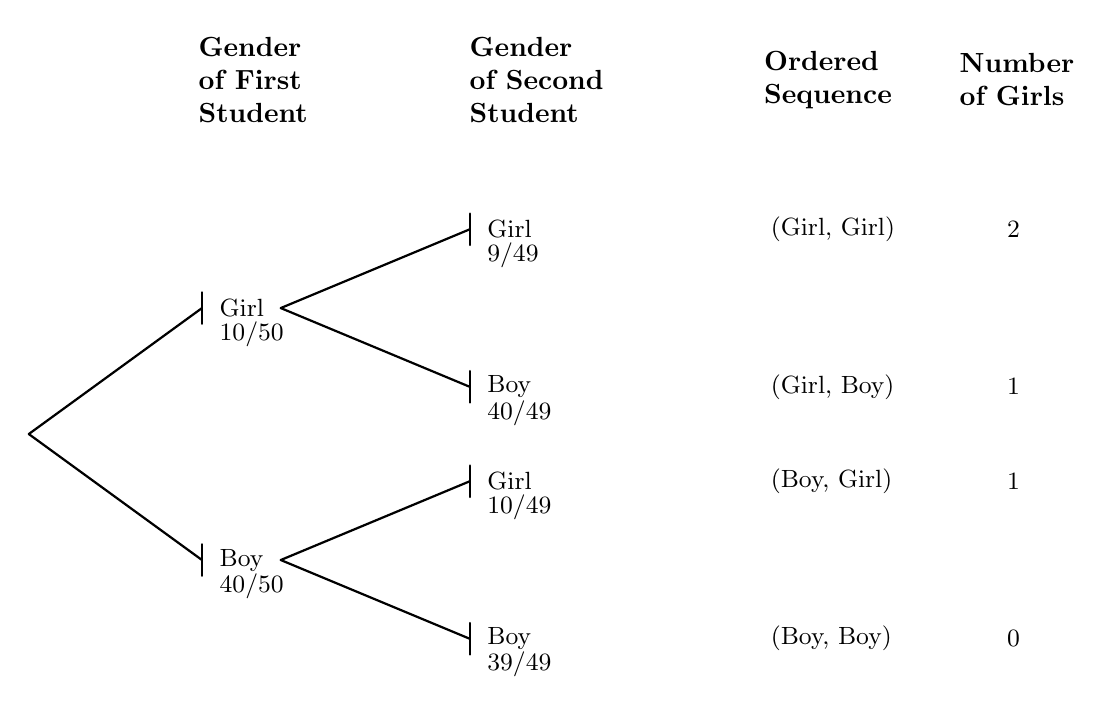
\begin{tikzpicture}[
  x=1cm,y=1cm,
  line cap=round, line join=round,
  font=\small
]

% =================================================
% A) THAM SỐ (CHỈNH Ở ĐÂY)
% =================================================
\def\xRoot{0.8}
\def\yRoot{0}

% vị trí các NÚT (tick) của lần chọn thứ nhất
\def\xFirst{3.0}
\def\dyFirst{1.6}

% vị trí các NÚT (tick) lá của lần chọn thứ hai
\def\xSecond{6.4}
\def\dySecond{1.0}

% khoảng chừa để ghi nhãn nút, và vị trí phân nhánh sau nút
\def\labGap{0.10}     % chữ cách tick sang phải
\def\afterNode{1.00}  % đoạn kéo dài sau nút tới junction (để chừa chỗ)

% tick
\def\tickFirst{0.2}   % tick cấp 1
\def\tickSecond{0.2}  % tick cấp 2

% tiêu đề + gạch chân
\def\titleY{4.5}
\def\titleXFirst{3.65}
\def\titleXSecond{7.25}
\def\ulYshift{0.65}   % độ hạ của gạch chân so với baseline title
\def\ulHalf{1.05}     % nửa độ dài gạch chân

% cột bên phải
\def\xSeq{10.1}       % cột "Ordered Sequence"
\def\xNum{12.6}       % cột "Number of Girls"
\def\titleXSeq{9.85}
\def\titleXNum{12.35}

% bố trí nhãn xác suất
\def\pYOffset{0.33}   % độ hạ của xác suất so với nhãn Girl/Boy

% =================================================
% B) ĐIỂM (NÚT + JUNCTION)
% =================================================
\coordinate (P)   at (\xRoot,\yRoot);

% Nút cấp 1 (tick đặt tại đây)
\coordinate (FirstGirl) at (\xFirst,{\yRoot+\dyFirst});
\coordinate (FirstBoy)  at (\xFirst,{\yRoot-\dyFirst});

% Junction sau nút cấp 1 (tách nhánh lần 2 ở đây)
\coordinate (JGirl) at ({\xFirst+\afterNode},{\yRoot+\dyFirst});
\coordinate (JBoy)  at ({\xFirst+\afterNode},{\yRoot-\dyFirst});

% Nút lá cấp 2 (tick đặt tại đây)
\coordinate (GG) at (\xSecond,{\yRoot+\dyFirst+\dySecond});
\coordinate (GB) at (\xSecond,{\yRoot+\dyFirst-\dySecond});
\coordinate (BG) at (\xSecond,{\yRoot-\dyFirst+\dySecond});
\coordinate (BB) at (\xSecond,{\yRoot-\dyFirst-\dySecond});

% =================================================
% C) VẼ CẠNH (đến nút -> qua junction -> tách)
% =================================================
% từ gốc đến nút cấp 1
\draw[thick] (P) -- (FirstGirl);
\draw[thick] (P) -- (FirstBoy);

% từ junction tách thành 2 nhánh đến các nút lá
\draw[thick] (JGirl) -- (GG);
\draw[thick] (JGirl) -- (GB);

\draw[thick] (JBoy) -- (BG);
\draw[thick] (JBoy) -- (BB);

% =================================================
% D) TICK (đặt tại NÚT, không đặt tại junction)
% =================================================
% tick cấp 1
\draw[thick] ($(FirstGirl)+(0,\tickFirst)$) -- ($(FirstGirl)+(0,-\tickFirst)$);
\draw[thick] ($(FirstBoy)+(0,\tickFirst)$)  -- ($(FirstBoy)+(0,-\tickFirst)$);

% tick cấp 2
\foreach \X in {GG,GB,BG,BB}{
  \draw[thick] ($(\X)+(0,\tickSecond)$) -- ($(\X)+(0,-\tickSecond)$);
}

% =================================================
% E) NHÃN NÚT + XÁC SUẤT (đúng như hình mẫu)
% =================================================
% ---- cấp 1
\node[anchor=west] at ($(FirstGirl)+(\labGap,0)$) {Girl};
\node[anchor=west] at ($(FirstGirl)+(\labGap,-\pYOffset)$) {$10/50$};

\node[anchor=west] at ($(FirstBoy)+(\labGap,0)$) {Boy};
\node[anchor=west] at ($(FirstBoy)+(\labGap,-\pYOffset)$) {$40/50$};

% ---- cấp 2
\node[anchor=west] at ($(GG)+(\labGap,0)$) {Girl};
\node[anchor=west] at ($(GG)+(\labGap,-\pYOffset)$) {$9/49$};

\node[anchor=west] at ($(GB)+(\labGap,0)$) {Boy};
\node[anchor=west] at ($(GB)+(\labGap,-\pYOffset)$) {$40/49$};

\node[anchor=west] at ($(BG)+(\labGap,0)$) {Girl};
\node[anchor=west] at ($(BG)+(\labGap,-\pYOffset)$) {$10/49$};

\node[anchor=west] at ($(BB)+(\labGap,0)$) {Boy};
\node[anchor=west] at ($(BB)+(\labGap,-\pYOffset)$) {$39/49$};

% =================================================
% F) TIÊU ĐỀ + GẠCH CHÂN (4 cột)
% =================================================
\node[align=left,font=\bfseries] at (\titleXFirst,\titleY)
  {Gender\\of First\\Student};
% \draw (\titleXFirst-\ulHalf,\titleY-\ulYshift) -- (\titleXFirst+\ulHalf,\titleY-\ulYshift);

\node[align=left,font=\bfseries] at (\titleXSecond,\titleY)
  {Gender\\of Second\\Student};
% \draw (\titleXSecond-\ulHalf,\titleY-\ulYshift) -- (\titleXSecond+\ulHalf,\titleY-\ulYshift);

\node[align=left,font=\bfseries] at (\titleXSeq+1.1,\titleY)
  {Ordered\\Sequence};
% \draw (\titleXSeq-\ulHalf,\titleY-\ulYshift) -- (\titleXSeq+\ulHalf,\titleY-\ulYshift);

\node[align=left,font=\bfseries] at (\titleXNum+1,\titleY)
  {Number\\of Girls};
% \draw (\titleXNum-\ulHalf,\titleY-\ulYshift) -- (\titleXNum+\ulHalf,\titleY-\ulYshift);

% =================================================
% G) CỘT "Ordered Sequence" + "Number of Girls" (căn theo lá)
% =================================================
\node[anchor=west] at (\xSeq, {0+\dyFirst+\dySecond}) {(Girl, Girl)};

\node[anchor=west] at (\xSeq, {0+\dyFirst-\dySecond}) {(Girl, Boy)};

\node[anchor=west] at (\xSeq, {0-\dyFirst+\dySecond}) {(Boy, Girl)};

\node[anchor=west] at (\xSeq, {0-\dyFirst-\dySecond}) {(Boy, Boy)};

\node[anchor=west] at ({\xNum+.5}, {0+\dyFirst+\dySecond}) {2};

\node[anchor=west] at ({\xNum+.5}, {0+\dyFirst-\dySecond}) {1};

\node[anchor=west] at ({\xNum+.5}, {0-\dyFirst+\dySecond}) {1};

\node[anchor=west] at ({\xNum+.5}, {0-\dyFirst-\dySecond}) {0};

\end{tikzpicture}
\end{document}
